

\section{Proteomik}
\subsection{Definition Proteomik} \index{Proteomik}
Das Proteom ist die quantitative Darstellung des gesamtenProteinexpressionsmusters einer Zelle, eines Organismus
oder eines Gewebes unter genau definierten Bedingungen
\subsection{Genom vs Proteom}
\begin{itemize}
    \item Das Genom ist statisch, da es durch die klare Abfolge von Nukleotiden definiert werden kann. \\
    Das Proteom ist dynamisch, weil sehr viele Parameter und Prozesse einfluss haben können!
    \item Das Genom sagt, was potentiell in einer Zelle passieren könnte, das Proteom sagt uns, was tatsächlich passiert.
\end{itemize}
\subsection{Was beeinflusst das Proteom?} \index{Proteom}
\begin{itemize}
    \item Pharmazeutische Substanzen
    \item Physiologie
    \item Stress
    \item Temperatur
    \item Zell-spezifische Gen-expression
    \item Kultur bedingungen
    \item Interaktionen
\end{itemize}
\subsection{Vorteile der Proteomik}
Experimentatoren arbeiten auf der Ebene der Genprodukte und beschäftigen sich mit
tatsächlich gebildeten Genprodukten und nicht mit Genen, die exprimiert werden undeine detektierbare mRNA bilden, aber nicht in ein Proteinprodukt translatiert werden.
\subsection{Voraussetzungen für die Proteomik}
Für den zu untersuchenden Organismus muß die komplette Genomsequenz oderzumindest eine Sammlung von vielen cDNA - Sequenzen bekannt sein.
\subsection{Limitierungen der Proteomik}
In der Regel kann in einem Proteomexperiment nicht die Gesamtheit der in einemOrganismus synthetisierten Proteine detektiert werden, wohingegen die Expressionaller Gene in einem Array- oder RNA-seq - Experiment verfolgt werden kann.
\section{Posttranslationale Modifikationen (PTMs)} \index{Posttranslationale Modifikation}
\subsection{Definition}
Als \glspl{ptm} bezeichnet man Veränderungen von
Proteinen, die nach der Translation stattfinden.
\section{2D Gelelektrophorese} 
Die 2D-Gelelektrophorese ist eine Methode zur Analyse komplexer Proteingemische. \index{2D-Gelelektrophorese}
\subsection{Erste Dimension}
Die erste Dimension, die isoelektrische Fokussierung (IEF), trennt Proteine aufgrund ihrer Ladung.\\
\glspl{Trägerampholyt} sind Gemische aus Hunderten verschiedener aliphatischer Oligo-Aminosäuren und Oligo-Carbonsäuren, die sich in ihren isoelektrischen Punkten unterscheiden.\\
Ein immobilisierter pH – Gradient (IPG) wird durch das kovalente Einfügen eines Gradientenaus sauren und basischen Gruppen in ein Polyacrylamidgel während des Gelgießens erzeugt.\\
\subsection{zweite Dimension}
Die zweite Dimension, Sodium Dodecylsulfat-Polyacrylamidgelelektrophorese (SDS-PAGE), trennt Proteine nach ihrem Molekulargewicht. \\
Effekte von SDS:
\begin{itemize}
    \item individuelle Ladungsunterschiede von Proteinen werden maskiert
    \item Wasserstoffbrückenbindungen werden aufgespalten
    \item hydrophobe Interaktionen werden aufgelöst
    \item die Aggregation von Proteinen wird verhindert
    \item Sekundärstrukturen von Proteinen werden aufgehoben
\end{itemize}
\begin{figure}[H]
    \centering
    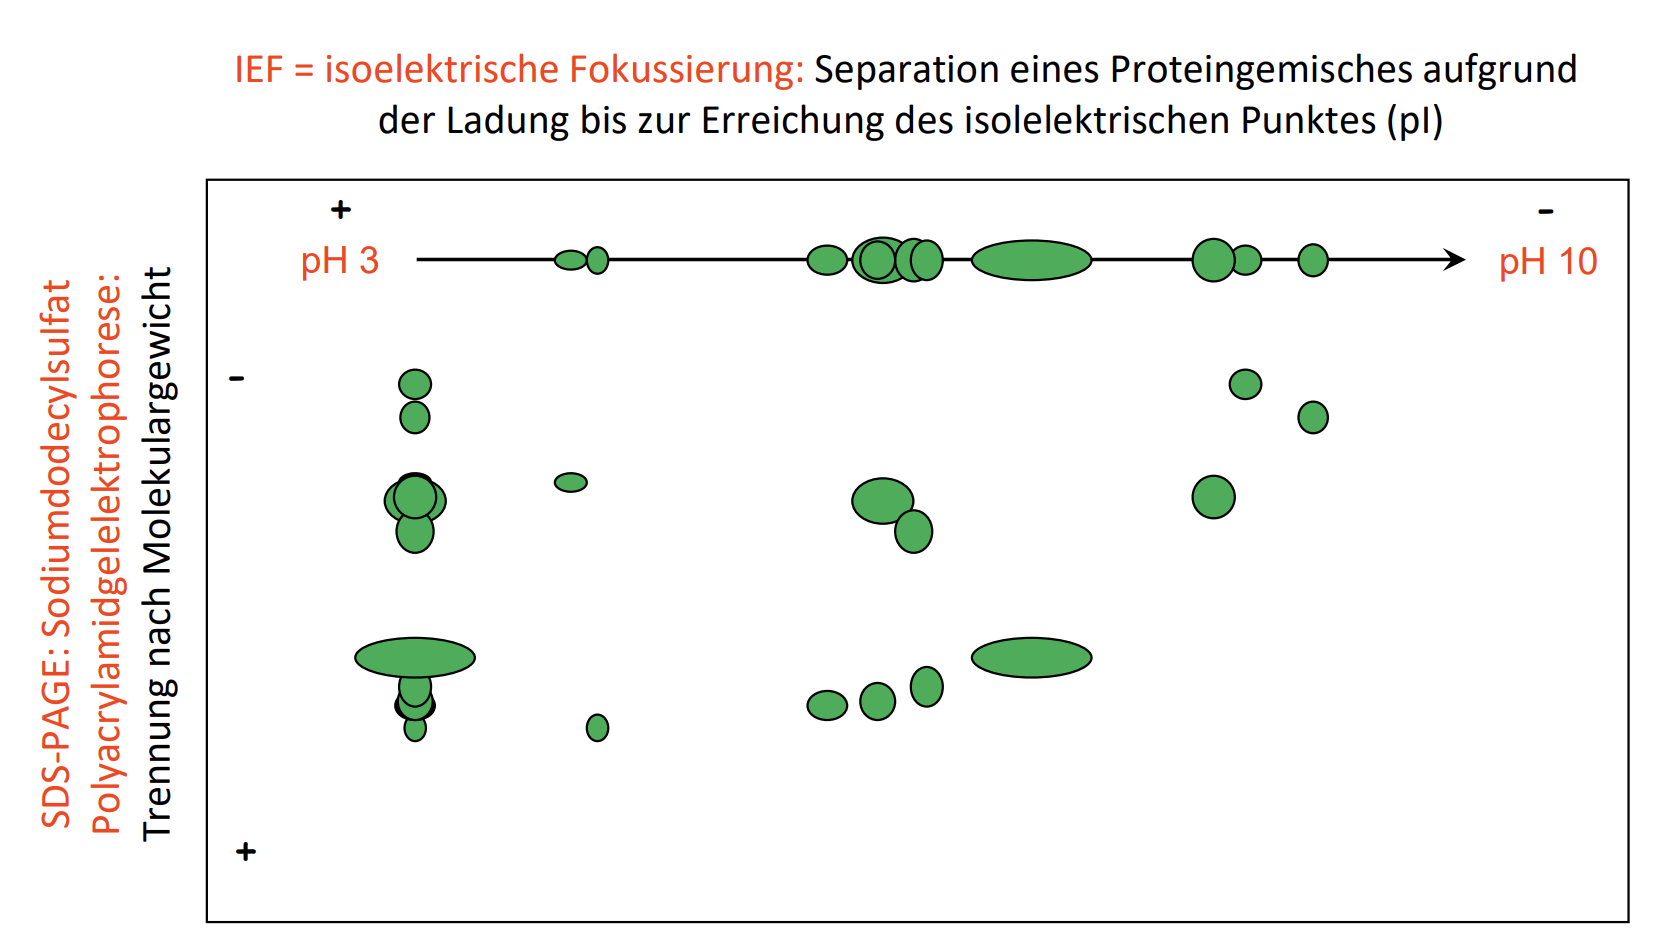
\includegraphics[width=0.8\linewidth]{images/2D Gelelektrophorese.png}
    \caption{Beispielgraphik einer 2D Gelelektrophorese}
    \label{fig:enter-label}
\end{figure}
\section{Proteine spalten}
Für viele Techniken der Massenspektrometrie müssen Proteine in Peptide
zerlegt werden, welche dann analysiert werden können.

\subsection{Trypsin}
\begin{figure}[H]
    \centering
    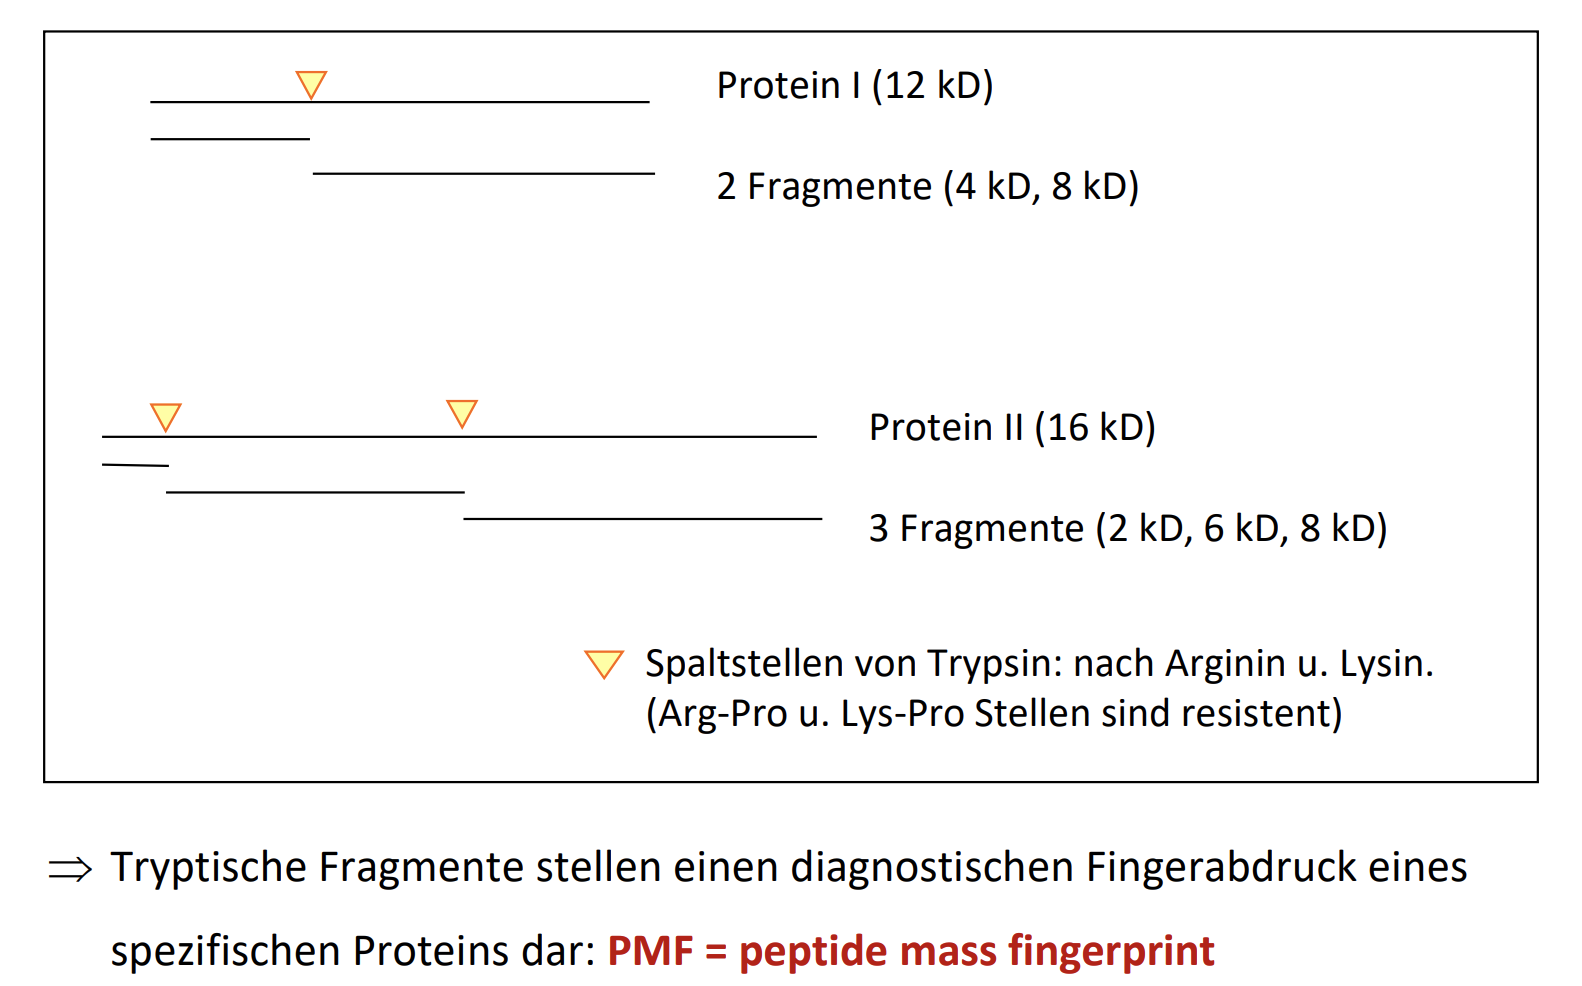
\includegraphics[width=0.8\linewidth]{images/Trypsinverdau.png}
    \caption{Spaltung von Proteinen mit Trypsin}
    \label{fig:enter-label}
\end{figure}
\section{Massenspektometrie} \index{Massenspektometrie}
\subsection{Aufbau}
\begin{itemize}
    \item Ionenquelle \\ 
    Hierbei werden die Proben in die einzelnen Ionen aufgelöst. Unterschiedliche verfahren werden hier angewandt wie MALDI.
    \item Massenanalysator \\
    Hierbei werden die einzelnen Ionen von einander durch häufig physische Gesetzte von einander getrennt. Die Masse ist der geläufigste Indikator zur Trennung der Ionen.
    \item Detektor \\
    Erfassung der unterschiedlichen Ionen und dessen Anzahl
\end{itemize}
\subsection{Matrix-assisted Laser Desorption/Ionization (MALDI)}
\begin{itemize}
    \item Nimmt ein Raster mit Proben entgegen
    \item desorbiert mit einem Laser die Proben in die einzelnen Ionen
    \item Einzelne Ionen gehen dann in den Massenanalysator.
\end{itemize}
\subsection{MALDI TOF} \index{MALDI TOF}
\begin{itemize}
    \item TOF = Time of flight
    \item Nach dem desorbieren der Proben werden die Ionen beschleunigt durch eine Elektrode
    \item Ionen fliegen dann durch ein Flugrohr in einen Detektor. \\
    Leichtere Ionen fliegen schneller in den Detektor als schwerere Ionen.
    \begin{itemize}
        \item Lineares Flugrohr \\
        Ist von der Form linear.
        \begin{figure}[H]
            \centering
            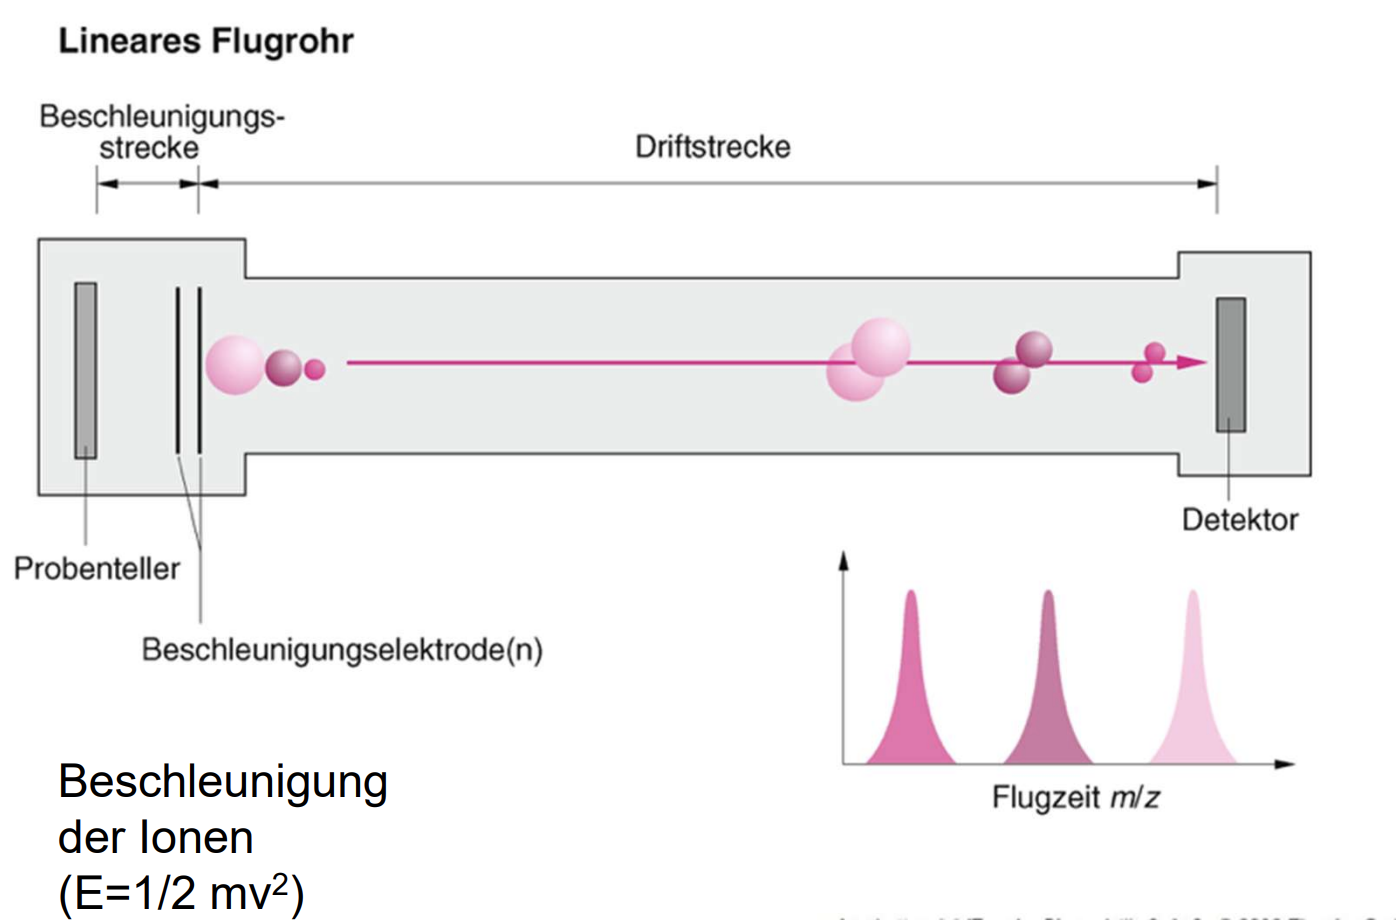
\includegraphics[width=0.8\linewidth]{images/lineares Flugrohr.png}
            \label{fig:enter-label}
        \end{figure}
        \item Reflektor flugrohr \\
        Reflektiert einmal die Ionen, sodass TOF länger ist.
        \begin{figure}[H]
            \centering
            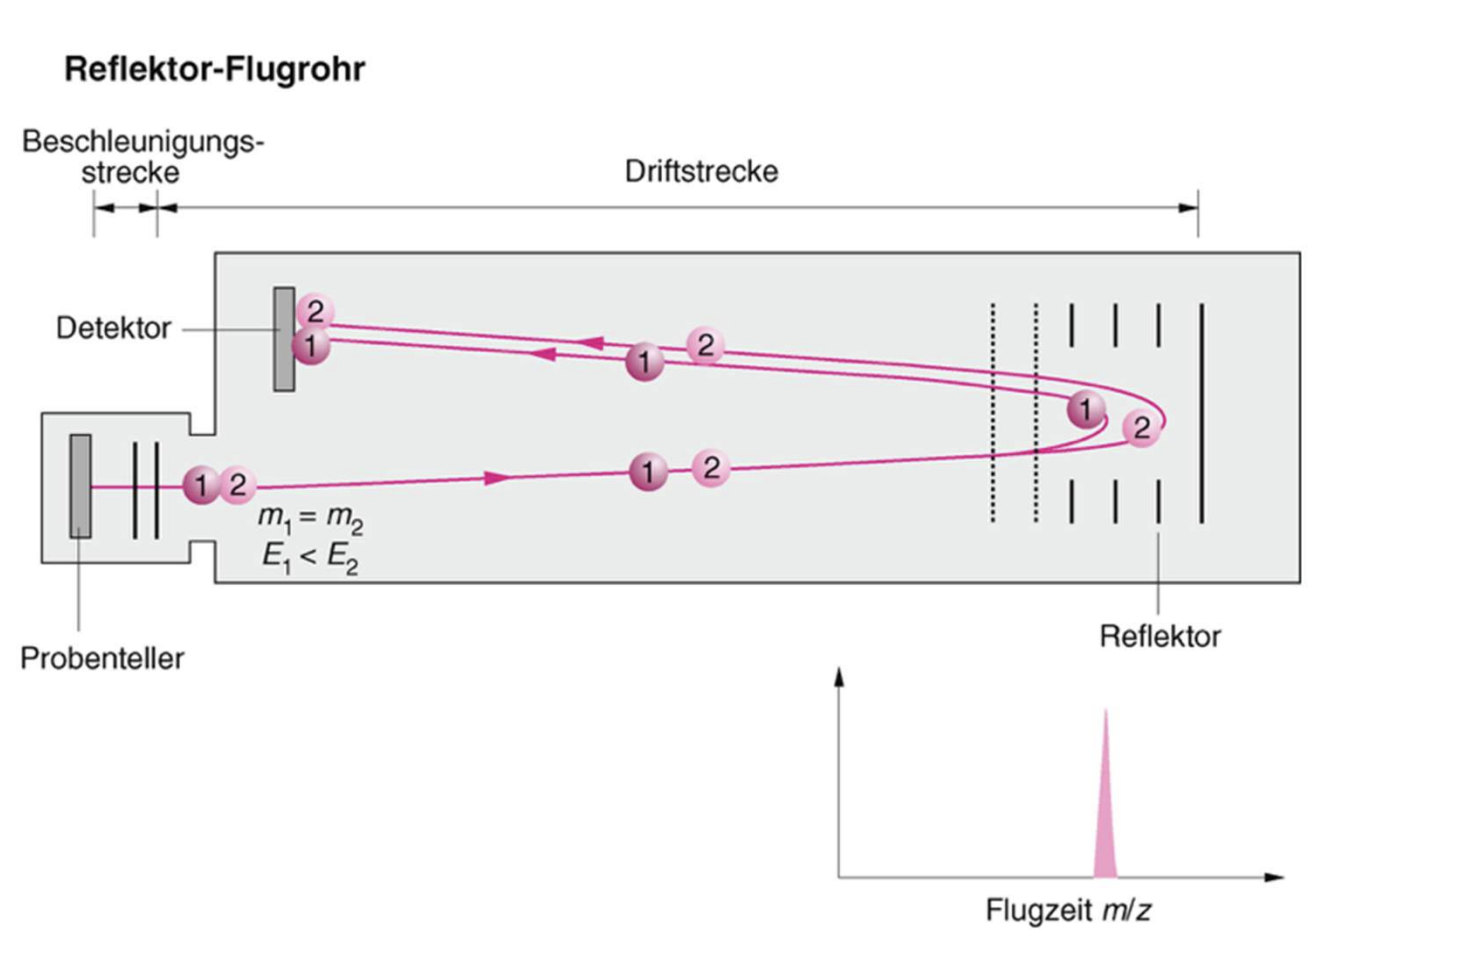
\includegraphics[width=0.8\linewidth]{images/Reflektor flugrohr.png}
            \label{fig:enter-label}
        \end{figure}
    \end{itemize}
\end{itemize}
\section{Electro Spray Ionisation (ESI)}
\begin{itemize}
    \item \textbf{Prinzip:} Eine Flüssigkeit wird in einem elektrischen Feld in viele kleine geladene Tröpfchen dispergiert.
    \item \textbf{Prozess:}
    \begin{itemize}
        \item Bildung geladener Tröpfchen.
        \item Lösungsmittelverlust führt zu erhöhter Ladungsdichte.
        \item Zerfall in Mikrotröpfchen.
        \item Desolvatisierung der Analytmoleküle.
    \end{itemize}
\end{itemize}
\begin{figure}[H]
    \centering
    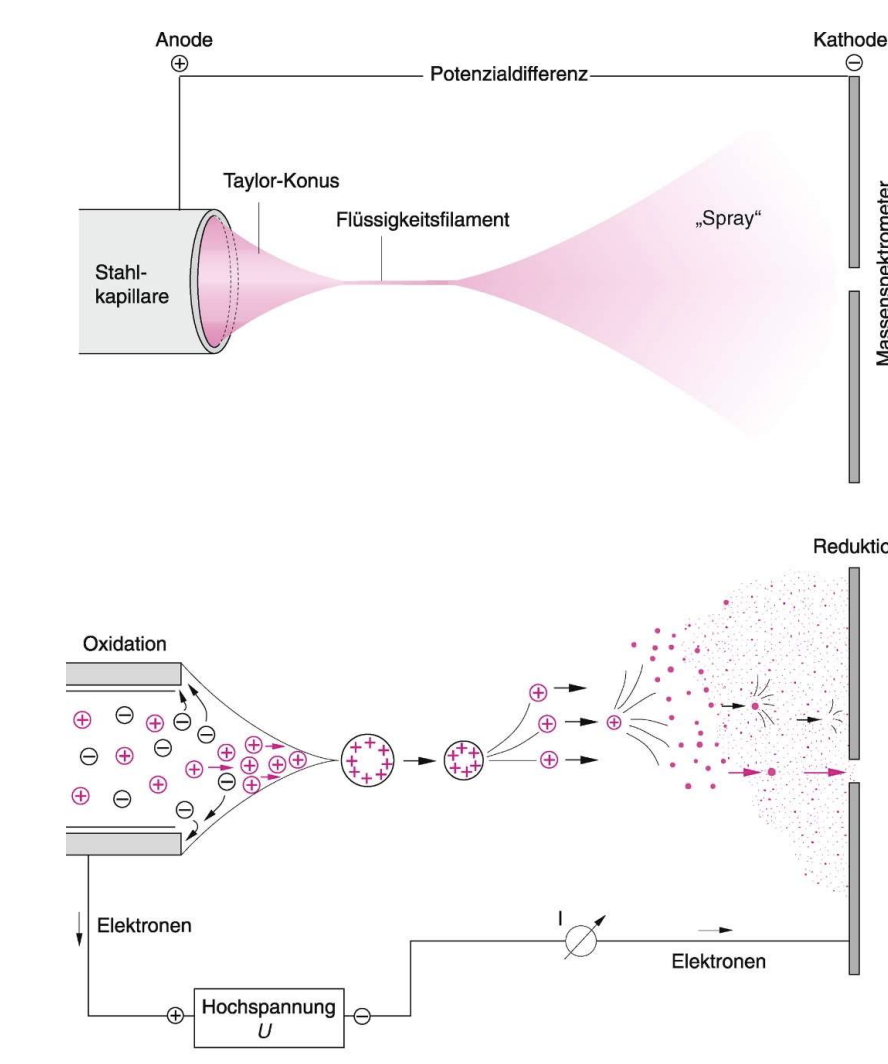
\includegraphics[width=0.8\linewidth]{images/ESI.png}
    \label{fig:enter-label}
\end{figure}

\section{Quadrupol-Analysator}

\begin{itemize}
    \item \textbf{Funktionsweise:} Ein elektrisches Feld aus Gleich- und Wechselspannung sorgt für die selektive Passage bestimmter Ionen.
    \item \textbf{Mechanismus:}
    \begin{itemize}
        \item Ionen mit passendem m/z-Verhältnis durchlaufen den Quadrupol in einer stabilen Bahn.
        \item Ionen mit zu hoher oder zu niedriger Masse werden instabil und aus dem Feld geworfen.
    \end{itemize}
\end{itemize}
\begin{figure}[H]
    \centering
    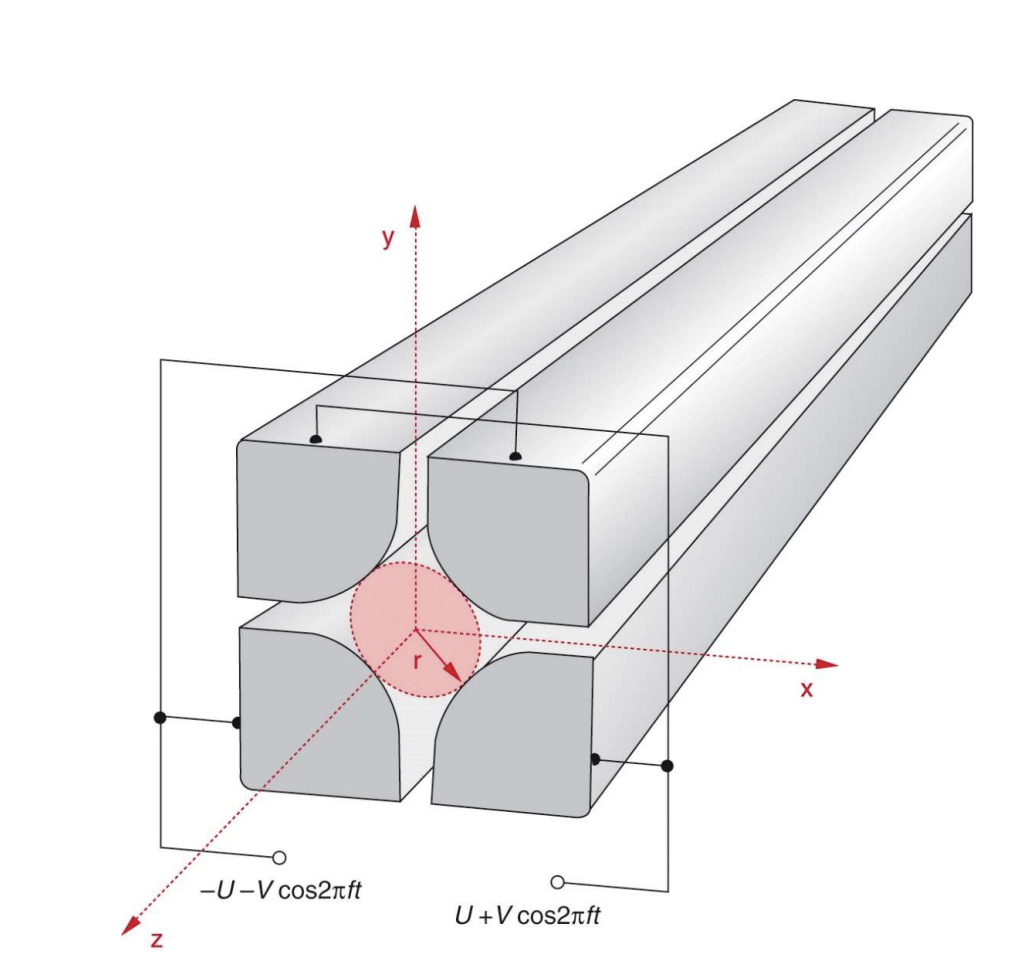
\includegraphics[width=0.8\linewidth]{images/Quadrupol Analyse.png}
    \label{fig:enter-label}
\end{figure}


\section{Quadrupol-Ionenfalle}

\begin{itemize}
    \item \textbf{Prinzip:} Ionen werden in einer Kombination aus hochfrequenten elektrischen Feldern und Gleichstrom gefangen.
    \item \textbf{Prozess:}
    \begin{itemize}
        \item Ionen oszillieren innerhalb des Feldes.
        \item Ein "Scanning"-Feld ejiziert Ionen mit bestimmten m/z-Verhältnissen für die Analyse.
    \end{itemize}
\end{itemize}
\begin{figure}[H]
    \centering
    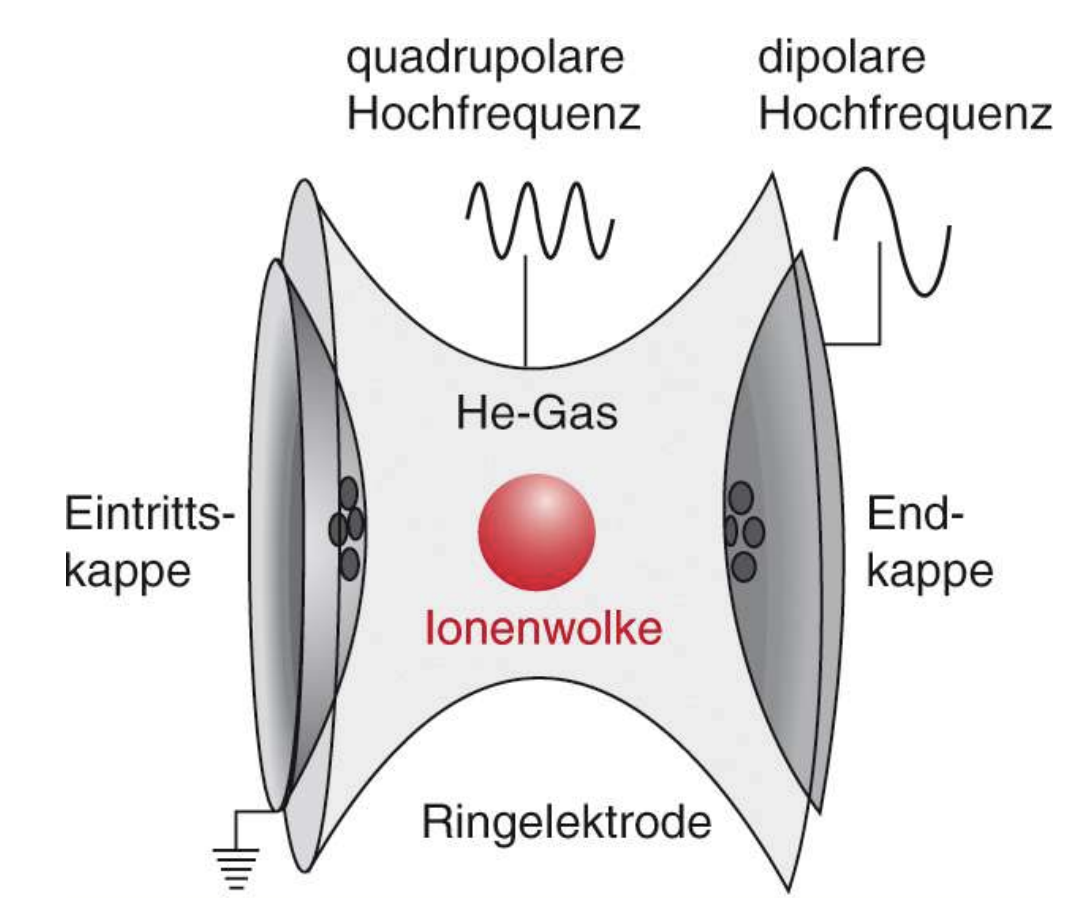
\includegraphics[width=0.8\linewidth]{images/Orbittrap.png}
    \label{fig:enter-label}
\end{figure}
\section{Orbitrap}

\begin{itemize}
    \item \textbf{Funktionsweise:} Ionen rotieren in einer Orbital-Ionenfalle um eine zentrale Elektrode.
    \item \textbf{Mechanismus:}
    \begin{itemize}
        \item Frequenz der Ionenschwingung ist proportional zu m/z.
        \item Fouriertransformation wird genutzt, um das Massenspektrum zu berechnen.
    \end{itemize}
\end{itemize}
\section{Tandem-Massenspektrometrie (MS/MS)}

\begin{itemize}
    \item \textbf{Prinzip:} Eine Kombination aus zwei Massenspektrometern zur gezielten Fragmentierung und Analyse von Molekülen.
    \item \textbf{Prozess:}
    \begin{itemize}
        \item Im ersten Massenspektrometer (MS1) werden Ionen nach ihrem m/z-Verhältnis separiert.
        \item Ein ausgewähltes Ion wird in einer Kollisionszelle fragmentiert (z. B. durch Stoß mit einem Inertgas).
        \item Die Fragmente werden im zweiten Massenspektrometer (MS2) analysiert.
    \end{itemize}
\end{itemize}
\begin{figure}[H]
    \centering
    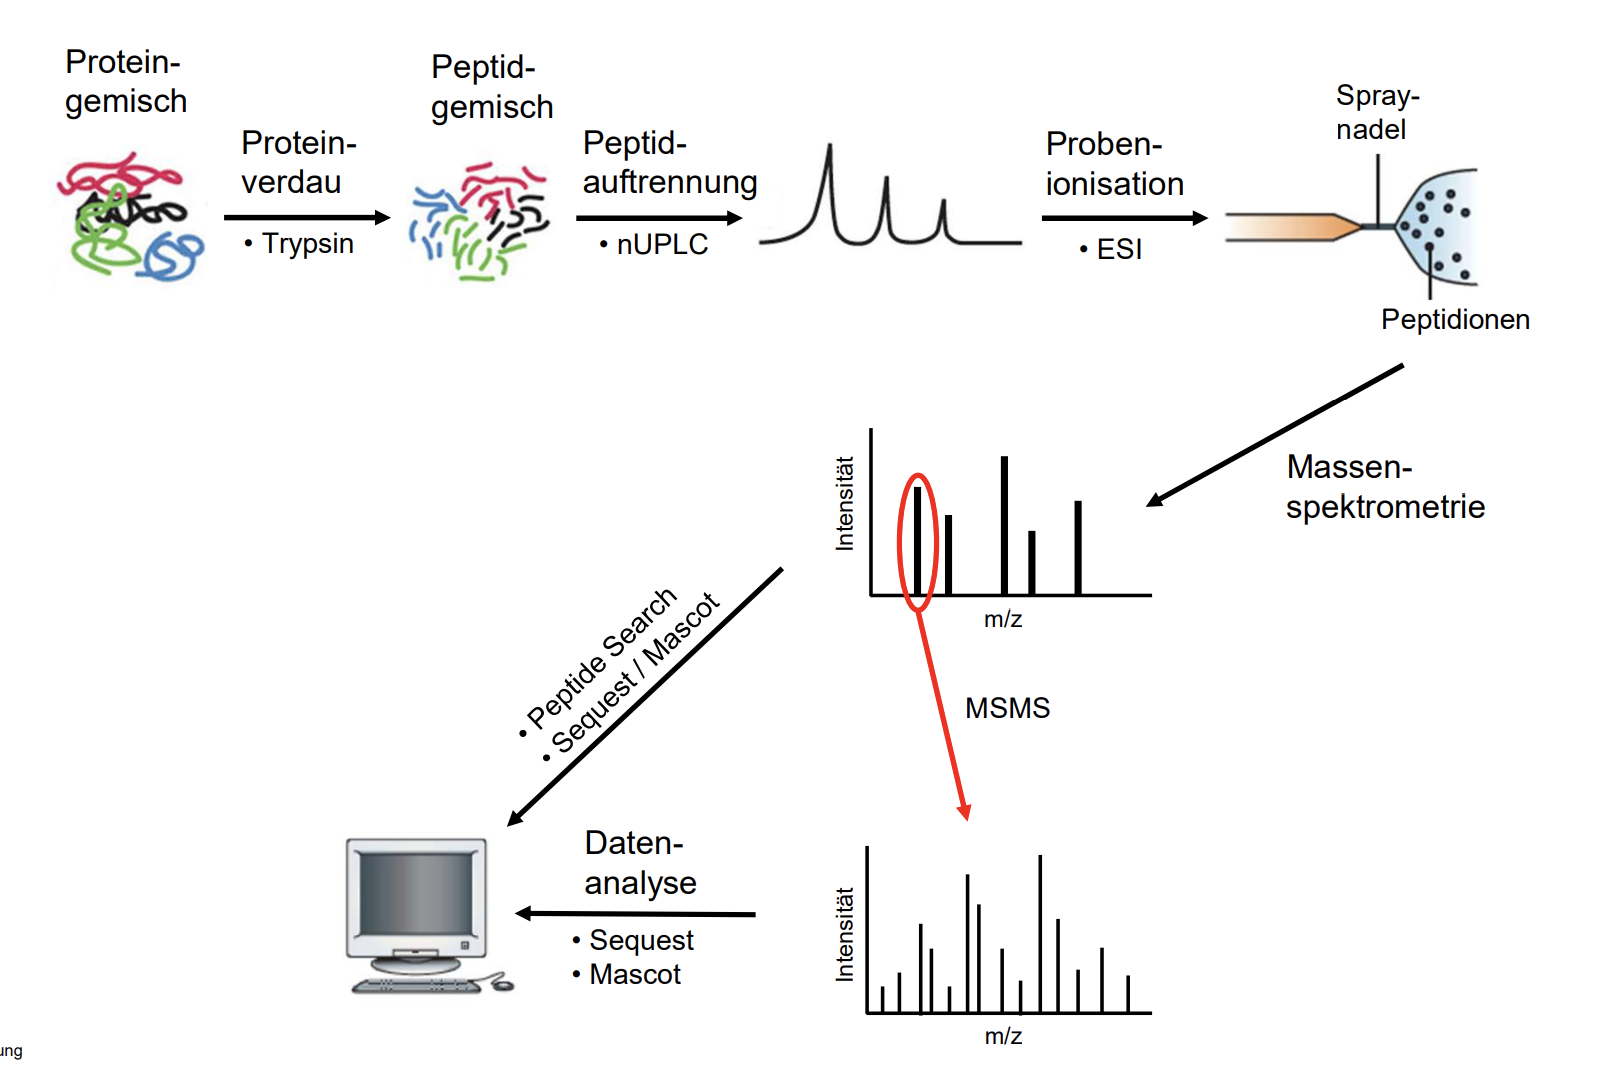
\includegraphics[width=1.0\linewidth]{images/Tandem Massenspektometrie.png}
    \label{fig:enter-label}
\end{figure}

\section{De novo Sequenzierung von Peptiden}

\begin{itemize}
    \item \textbf{Definition:} Methode zur Bestimmung der Aminosäuresequenz eines Peptids, ohne dass eine Referenzdatenbank benötigt wird.
    \item \textbf{Prinzip:}
    \begin{itemize}
        \item Ein Peptid wird fragmentiert, typischerweise durch Collision-Induced Dissociation (CID) oder Electron Transfer Dissociation (ETD).
        \item Die entstehenden Fragmentionen werden analysiert, um ihre Massenunterschiede zu bestimmen.
        \item Diese Massenunterschiede entsprechen spezifischen Aminosäuren und ermöglichen die Rekonstruktion der Peptidsequenz.
    \end{itemize}
    \item \textbf{Nomenklatur der Fragmentionen:}
    \begin{itemize}
        \item \textbf{b-Ionen}: Entstehen durch Spaltung der Peptidbindung und behalten den N-Terminus.
        \item \textbf{y-Ionen}: Entstehen durch Spaltung der Peptidbindung und behalten den C-Terminus.
    \end{itemize}
\end{itemize}

\begin{mechanism}[title=Definition PMF]
"Peptid massen fingerabdruck" (peptid mass fingerprint) \\
Mit hilfe von selektiven Proteasen (bspw. \gls{Trypsin}) und MS können die massen der einzelnen peptide von Proteinen ermittelt werden. Die Summe der Massen entspricht der Proteinmasse. Jedes Protein hat ein einzigartige masse.
\end{mechanism}
\begin{mechanism}[title=Wie erhält man PMF und was stellt es dar?]
PMF stellt die einzigartige Masse von einem Protein dar. Die Ermittlung solcher Masse funktioniert wiefolgt: \\
Das Protein wird in einem SDS-Gel mit selektiven Proteasen verdaut. Das Produkt sind dann die Einzelnen fragmente / peptide des Proteins. Anschließend kann durch \gls{ms} die Masse der einzelnen Peptide ermittelt werden. Die Summe solcher ist dann die Masse des Proteins, welche einzigartig ist.
\end{mechanism}

